% !TEX root = thesis.tex

%
%\begin{figure*}[t]
%	
%	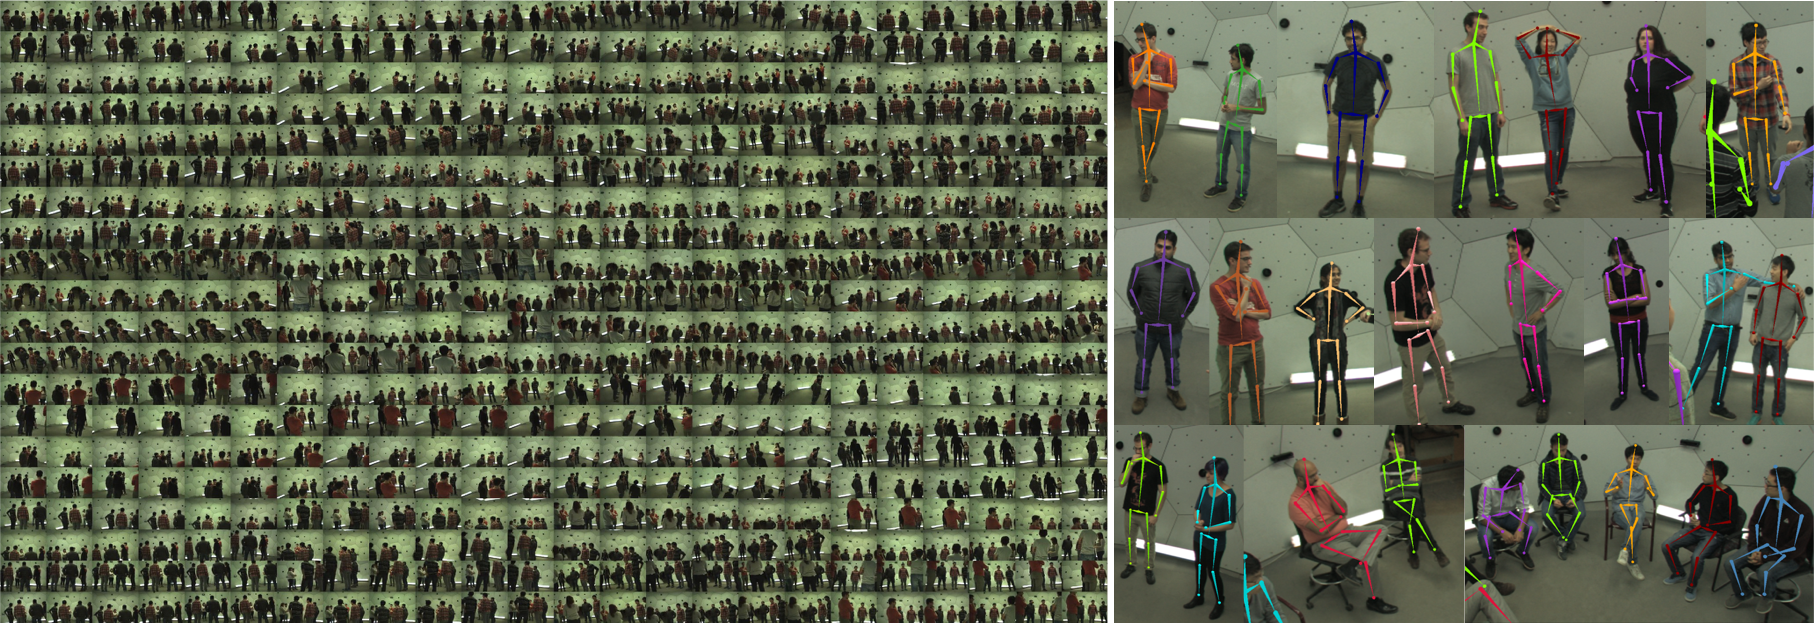
\includegraphics[width=\linewidth]{imgs/Teaser_0814}
%	\caption{(Left) 480 unique VGA views capturing a social interaction within the Panoptic Studio. (Right) HD example views showing frequently occurring postures that carry rich social signals, with 3D body pose automatically annotated by our method.} 
%	\label{fig:iconicPoses}
%\end{figure*}

\chapter{Introduction}
\label{sec:introduction}
\begin{figure}[h]
	 	
%	\caption{Kinesic signals play important roles in social communication to transmit messages that cannot be conveyed by verbal languages. In this thesis proposal, we present a system and method to measure full body kinesic signals including anatomical landmarks from body, face, and hands. We also propose an approach to model kinesic signals in social interaction by optimizing a prediction function in continuous high bandwidth kinesic signal space.}	
	\label{fig:intro}
\end{figure}

%Kinesics signal is important
During our daily communication, we use our body, hands, and faces to convey our thoughts, intentions, and emotions (as shown in Figure~\ref{fig:intro}). These signals transmitted by our body motion are often elaborate; a subtle changes in the motion can transmit a completely different meaning. As a human, we are extremely familiar with how to use these signals in a social communication---we encode our internal messages to the form of the signals and interpret the transmitted signals from others by decoding them appropriately. This encoding and decoding processes are continuously performed in our communication, and play an essential role in conveying messages that cannot be fully transmitted by verbal language.  

``Kinesics" is a term that refers to the study of body movements and gestures used in social communication, and includes the interpretation of facial expressions, hand gestures, and gaze movements\footnote{The term ``body language" is also used to refer to the same meaning in non-scientific literatures.}. The specific term was first introduced and pioneered by Birdwhistell~\cite{Birdwhistell52,Birdwhistell-1970}, although interest in analyzing body movements for nonverbal communications goes back centuries (e.g., Aristotle, 330 BC)~\cite{dael2015measuring}. Understanding Kinesic signal is an essential part to understanding human, which is also closely related to many scientific fields including robotics, artificial intelligence, and virtual reality, towards making an artificial agent that can genuinely interact with humans. 

%Since then, kinesics have become significant in understanding nonverbal communication of humans, receiving sustained attention from many fields of scientific inquiry. 

However, kinesics is still a largely unexplored area. Although we are extremely accustomed to using kinesic signals for our daily communication, we are incredibly ignorant in explicitly defining the underlying protocol of the signals. The kinesic signals are emitted from movements or postures of any part of the body or the body as a whole. A combination of subtle movements from body parts such as fingers, eyebrows, gaze, and shoulders can have a different meaning in different contexts. Furthermore, the signals exist in a continuous spatio-temporal space, and do not have boundaries for a clear segmentation. Due to this complexity, kinesic signals are hard to measure, describe, and understand. Our limited understanding of the kinesic signals and the protocol to encode and decode them makes it hard to transfer the ability to machines or artificial intelligence. As a result, machines are still completely blind to these signals; there is no machine or robot which can genuinely interact with humans with kinesic signals by understanding the meaning of our body gestures and using the similar signals to express its own intention and emotion. 


%While we have observed a great success in natural langauge processing with several commercial system and demos

% In most prior work, it is required that well trained human annotators spend time to manually describe a discrete number of events or motions by analyzing videotaped scenes~\cite{harrigan2013methodology, dael2015measuring}. This approach is not only labor-intensive, but also hard to objectively standardize, and more importantly it cannot represent all the subtlety expressed by kinesic signals due to its limited representation power. Describing kinesic signals using a few hand-crafted codes means projecting the original dimension defined in a continuous spatio-temporal domain into a discrete and quantized space. Thus, despite many existing approaches to build a manual coding system to functionally and anatomically describe kinesic signals in social communication~\cite{Ekman-1977, van2014body, harrigan2013methodology, dael2015measuring}, these approaches are fundamentally limited in objectively and accurately modeling them. 

The objective of this thesis is to further our understanding of kinesics signals in social communication based on a data-driven and computational approach, aiming to endow ``kinesic signal processing" ability to machines. As major advancements in science are nearly always preceded by innovations in engineering that enable us to measure the world, the first part of this thesis starts by presenting a system and method to measure such signals. As a core contribution, a massively multiview capture system, the \emph{Panoptic Studio}, is built to capture naturally interacting people in social situations. Methods to measure the subtle movements of anatomical landmarks including facial expression, hand gestures and body motions are also presented. The novel measurement system and methods enable to build a 3D deformation model to capture the ``total body motion" in a unified parametric space. To this end, a large scale dataset containing 3D kinesic signals of hundreds of participants is collected. Our dataset includes the full spectrum of kinesic signals of naturally interacting people, as well as the corresponding input data from more than 500 sensors.% at high resolution where subtle body movements  including facial expressions and hand gestures are captured in a markerless way. %This dataset enables us to model kinesic communication by a data-driven way. 

Based on the large scale dataset we have collected, we present an approach to model kinesic communication as information flow between coupled agents that continuously predict each others' response signals. In our method, a model takes kinesic signals transmitted by other people as input and ``predicts" the response kinesic signals of the target person as output. The core theme of our approach is that a meaningful encoding of body movement will emerge from representations that are optimized for efficient prediction of these kinesic communication signals. Our large scale dataset enables us to perform such optimization in the continuous high dimensional signal spaces. As a core discovery, we quantify the amount of information conveyed by each part of kinesic signanls (e.g. face vs. hand vs. body) and compare their importances in the social communication perspective, by using the prediction performance by a discriminative model as a quantity measure. %This thesis can be We believe this thesis presents a for the first time in the history.   %This approach becomes possible by the full spectrum of social signals  measruemneobtained from our system. %In this thesis, we explore this approach by predicting continuous facial gaze directions of a participant in triadic social situations.


%Quantity of Information

%Shannon, Ralph Hartley

%https://plus.maths.org/content/information-surprise


 %Our goal is to train a kinesic communication model to behave similar to humans in socials situations; given the kinesic signals it takes, our model produces kinesic signals similar to the ground truth signals measured in our dataset. This can be considered as a step to build an artificial agent that can communicate with humans using kinesics signals. %To this end, we also propose a way to quantify influence of each body part in social communication.

%%% Old version
%
%%Social Signal is important
%We, as social beings, live in the world surrounded by family, friends, colleges, and acquaintances. Social communication is the means of connection between people, and various social signals including verbal languages and body gestures are used for communication to share an individual's thoughts, intents, and emotions. Social communication is necessary at any moment when people share their time or space with others. Face-to-face interaction is the most obvious example occurring where people are strongly engaged in the communication, and, more generally, other situations where people are not directly engaged but affect each other can be also included in a form of social communication. For example, people avoid collisions with other pedestrians when they walk on the street, and people stand as far from each other as possible in an elevator. Although in these examples they are not explicitly communicating via verbal language, some type of social signals (position and appearance in these examples) emitted by other people still transmit important information, and people' motions are affected by them to live in the same world together. Social interactions occur very frequently in our daily life, and, due to their importance, understanding how humans socially communicate each other is essential to understand human and is also central to various research fields including psychology, sociology, human-computer interaction, robotics, and artificial intelligence.  
%
%Social communication can be divided into verbal and nonverbal communication. The verbal communication is based on words, and the nonverbal part means all types of ``other-than-words" signals, including facial expressions, body gestures, distance between people~\cite{Hall66}, relative position~\cite{kendon90}, prosody, physical appearance, and so on. Compared to the verbal part,  the nonverbal communication is relatively poorly understood, although increasing evidence show that it is as important as the verbal counterparts. For example, it is commonly accepted by social psychologists that much of the emotional meaning is expressed via nonverbal signals \cite{Mehrabian67, Mehrabian81, Birdwhistell70, Moore13}. Interestingly, although we are extremely accustomed to using these signals, we are incredibly ignorant in defining them. While we are often taught how to use verbal communications (speaking, listening, and writing) in our education system, it is extremely rare to teach or be taught about how to nonverbally communicate with others. For example, it is hard to describe which facial expressions and body gestures should be used during a specific situation. The major reason is that we do not fully understand it yet and we do not know how to transfer the knowledge to others---Sapir~\cite{Sapir-1949} called it ``an elaborate code that is written nowhere, known to no one, and understood by all". Compared to the area such as natural language processing area and computer vision, the nonverbal communication is still largely unexplored, and, consequently, robots or machines that can use expressions and gestures to genuinely interact with humans do not exist.
%
%Why is the study of nonverbal interaction still in its infancy, despite the centuries of research? To computationally study nonverbal social interactions, the data should be captured and measured first. However, unlike verbal signals that can be losslessly converted to languages, it is unclear how to capture, measure, and represent nonverbal signals. It is also poorly explored about how to analyze the social interaction related to the nonverbal signals. The dimension of social signals are high, and they exist in a continuous space. They cannot be further annotated by simpler forms (e.g., a few manually defined categories at quantized levels) rather than the measured signal themselves because a large amount of subtle information should be missing in the low level representation. %Thus supervised machine learning techniques are hardly applicable since the data cannot be objectively Given the fact that our internal status cannot be objectively measured, how we can understand and analyze social signals and social interactions is not a straightforward problem, if the social signals can be measured at all.    
%
%\begin{figure}[t]
%	\centering
%	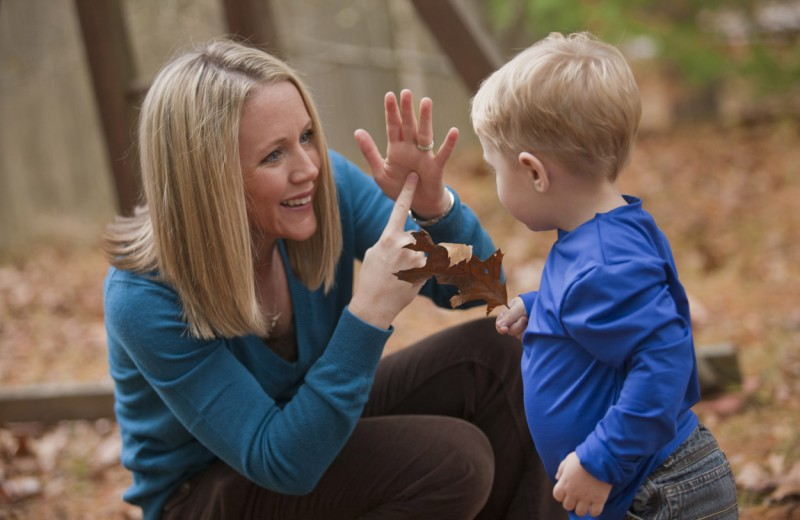
\includegraphics[trim=0 0 0 0, clip=true, height=0.2\columnwidth]{figures/intro_1}
%	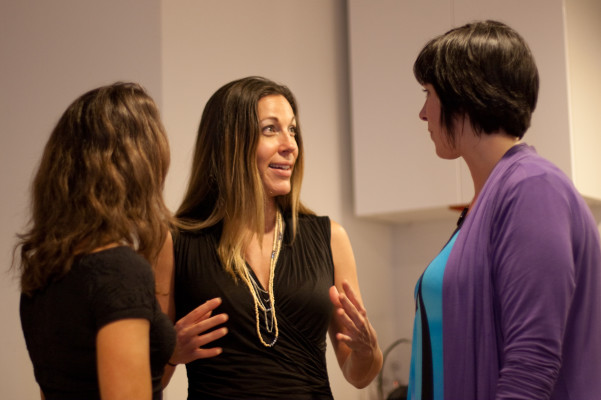
\includegraphics[trim=0 0 0 0, clip=true, height=0.2\columnwidth]{figures/intro_5}
%	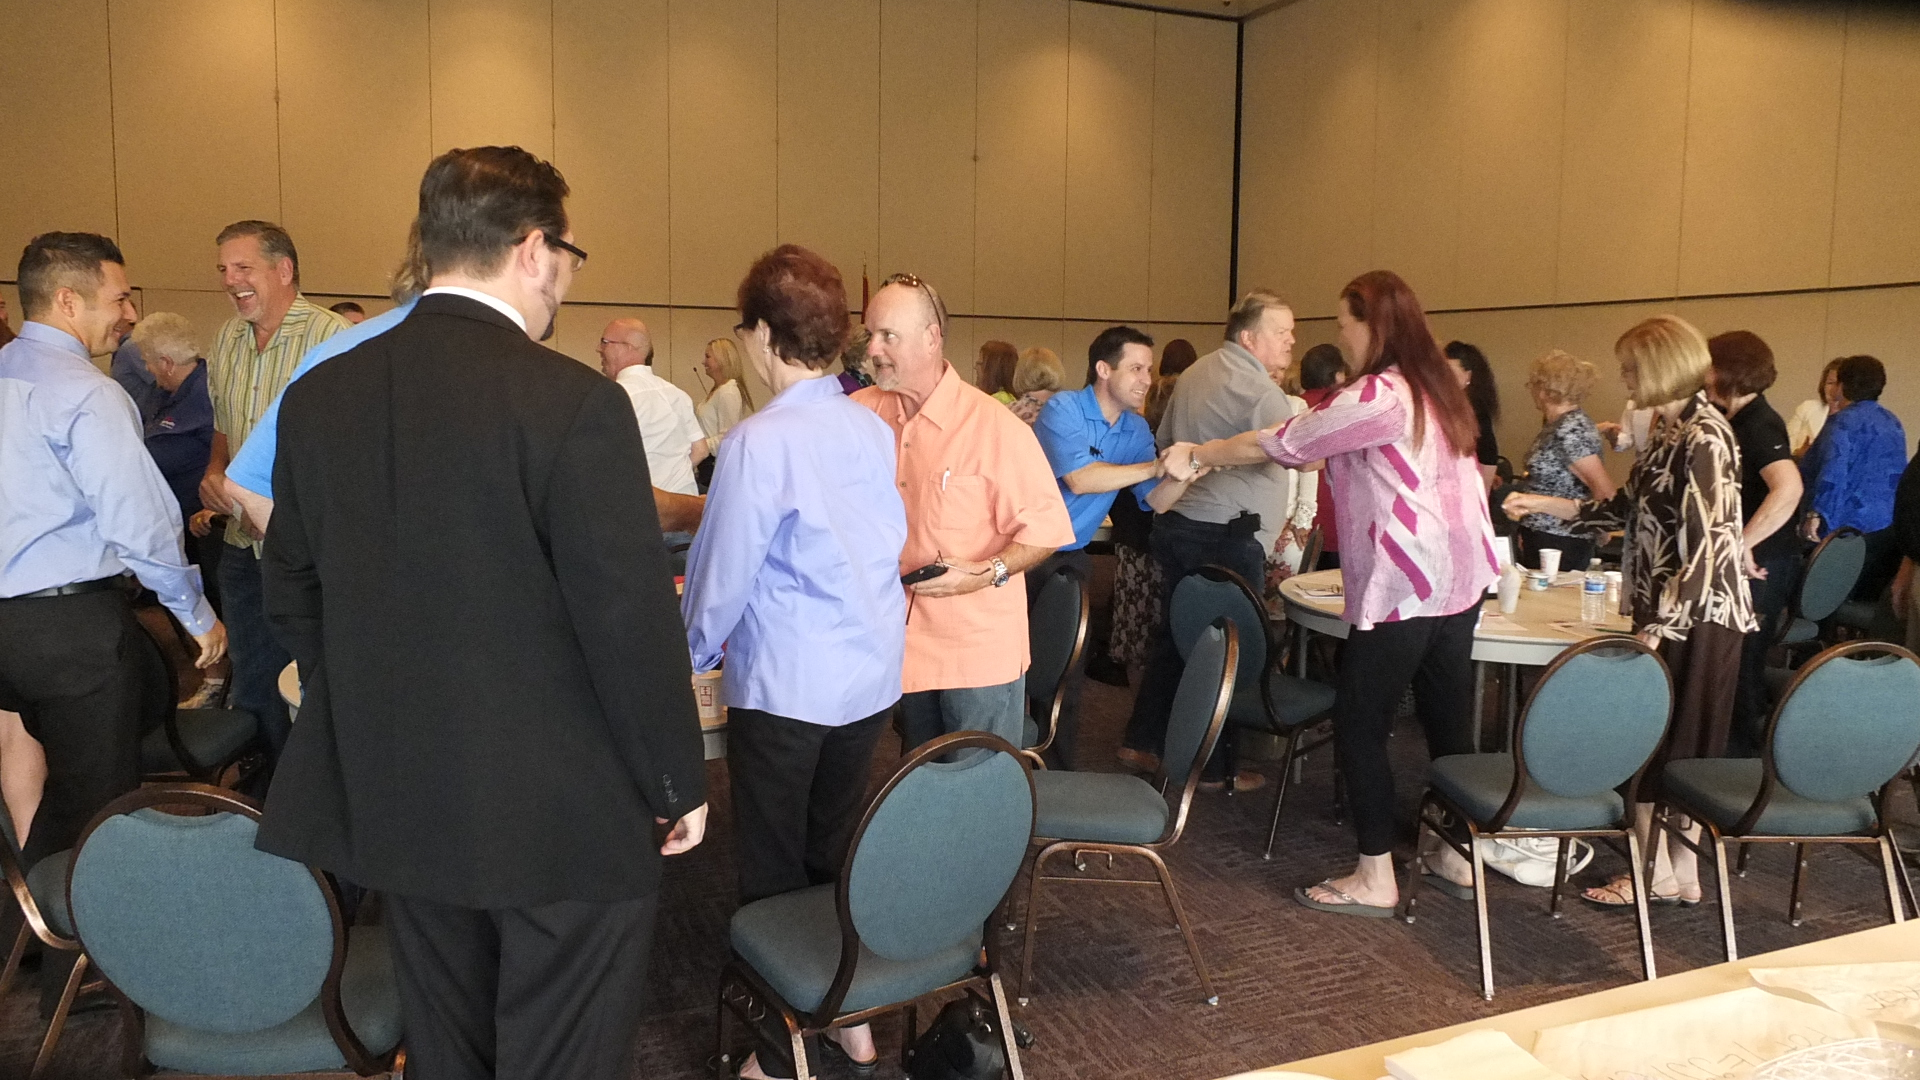
\includegraphics[trim=0 0 0 0, clip=true, height=0.2\columnwidth]{figures/intro_3}
%	\caption{We communicate each other using various social signals. To study this, multiple challenges to capture, measure, and understand social signal and interactions should be addressed.}	
%	\label{fig:intro}
%\end{figure}
%
%The objective of this thesis is to understand nonverbal communication of interacting people in a data-driven way. This thesis mainly focuses on the signals that can be obtained by visual information. As all past Scientific discoveries often begin by presenting novel measurement methods, the first part of this paper starts by presenting a system and methods to capture and measure social signals. As a core innovation, a massively multiview capture system, the Panoptic Studio, is built for this specific goal. Algorithms to measure subtle social signals in different body landmarks are presented by fully utilizing our system with minimum priors about scenes. A large scale dataset capturing hundreds of naturally interacting people is built playing social game designs. To this end, we present a framework to computationally analyze social interaction in a form of social signal prediction, and multiple novel scientific discoveries in understanding nonverbal social interaction are address.  

\section{Challenges}
This thesis aims to computationally analyze kinesic signals. To achieve the goal, the signals naturally emerging from interacting people should be obtained first. However, it is challenging to capture and measure such signals in social situations due to multiple challenges addressed in this section. The lack of existing data limits the opportunity to computationally model kinesic communication, causing a singular focus on limited measurements and scenarios (e.g., face only, a table setup allowing limited body motions, and dyadic communication only). In this thesis, two major challenges in pursuing computational analysis of kinesic signals are addressed.\\ % . 

\noindent \textbf{How To Measure Kinesic Signals}:  
During social interactions, strong occlusions emerge functionally (e.g., people systematically face each other while interacting, bodies are occluded by gesticulating limbs). Due to this reason, a single view cannot capture the entire social signals of multiple people. For example in Figure~\ref{fig:intro}, only a subset of the faces and body gestures of a part of people are captured from the camera view. To accurately analyze social interactions, a volume sufficient to house a social group should be assumed, yet all the subtle details of the motion where important social signals are embedded must be captured. A laboratory setup with multiple cameras is preferred to achieve this objective, and it is expected that the sensing challenges can be reduced according to increasing unique view points. However, in most prior work, a few cameras are often used, and, thus, limited research directions are only considered, for example: (1) studies only focus on face signals ignoring body motions~\cite{messinger2009automated, lucas_trust_2016,mckeown2012semaine}; (2) studies consider situations in a table setup where participants' motions are limited~\cite{carletta2005ami, Lepri-12,messinger2009automated, nojavanasghari2016emoreact, lucas_trust_2016,mckeown2012semaine}; (3) studies assume only few number of people (e.g., dyadic communications)~\cite{messinger2009automated,nojavanasghari2016emoreact, lucas_trust_2016, katsimerou2016crowdsourcing,mckeown2012semaine,gunes2006bimodal}.

%\noindent \textbf{How To Measure Kinesic Signals}:  
For computational analysis, captured raw data (images or videos) should be semantically labeled. For example, a human can infer 3D structure of other people and perceive movements of their anatomical landmarks (e.g., mouth, hands, eyes, and so on). Similarly, it is necessary to measure these semantics of kinesic signals from captured images and videos to make machines to decode their meaning. Importantly, these kinesic signals should be measured non-intrusively to avoid potential primes in natural interactions, and, thus, artificial markers or a specialized suit often used in motion capture system should not be exploited. Markerless motion capture in computer vision tackles this challenge, but most previous work is demonstrated in the scenes that are far from social situations, often capturing a single subject only, and assuming a predefined 3D template for each individual~\cite{Gall-09, Vlasic-08, Brox-10, Stoll-11, deAguiar-2008, Vlasic-2008}. Motions from faces and hands that play an important role in social interactions are rarely measured in social situations.\\

\noindent \textbf{How To Model Kinesic Signals}: 
It is unclear how to modeling kinesic signals by a data driven way. Even if we assume that the measurements of kinesic signals are provided, there is no way to objectively represent underlying social meaning of the signals. For example, a smile signal, formed by flexing the muscles at the side of the mouth with a contraction of the muscles at the corner of the eyes, may represent a happiness. However, the internal emotion expressed by the measured signals cannot be simply annotated by a ``smile" or ``happiness", because it may have a variety of subtly different meanings and intensities depending on the spatial and temporal variations of the facial movements. The Figure~\ref{fig:kinesicflow} describes an information flow in kinesic communication between individuals, where an encoding and a decoding between signals and messages are continuously performed. Most prior work is focused on deciphering the encoders and decoders between signals and the messages, which are often annotated into a few discrete categories~\cite{pantic2000automatic,cowie2001emotion,shan2009facial,cowie2001emotion,gunes2006bimodal}. These approaches, however, are fundamentally limited, because we cannot objectively measure or represent the internal status (e.g., the messages conveyed by signals and their interpretations in Figure~\ref{fig:kinesicflow}), but only can measure the exposed signals themselves.

%Prior work annotate social signals (e.g., face landmarks and EMG sensor output) by a few manually defined categories in quantized degrees (e.g., sentiment), but it basically assumes a mapping from the high dimensional continuous signals to a low dimensional discrete space, losing large amount of subtle details of signals.\\

%	\begin{figure}[t]
%		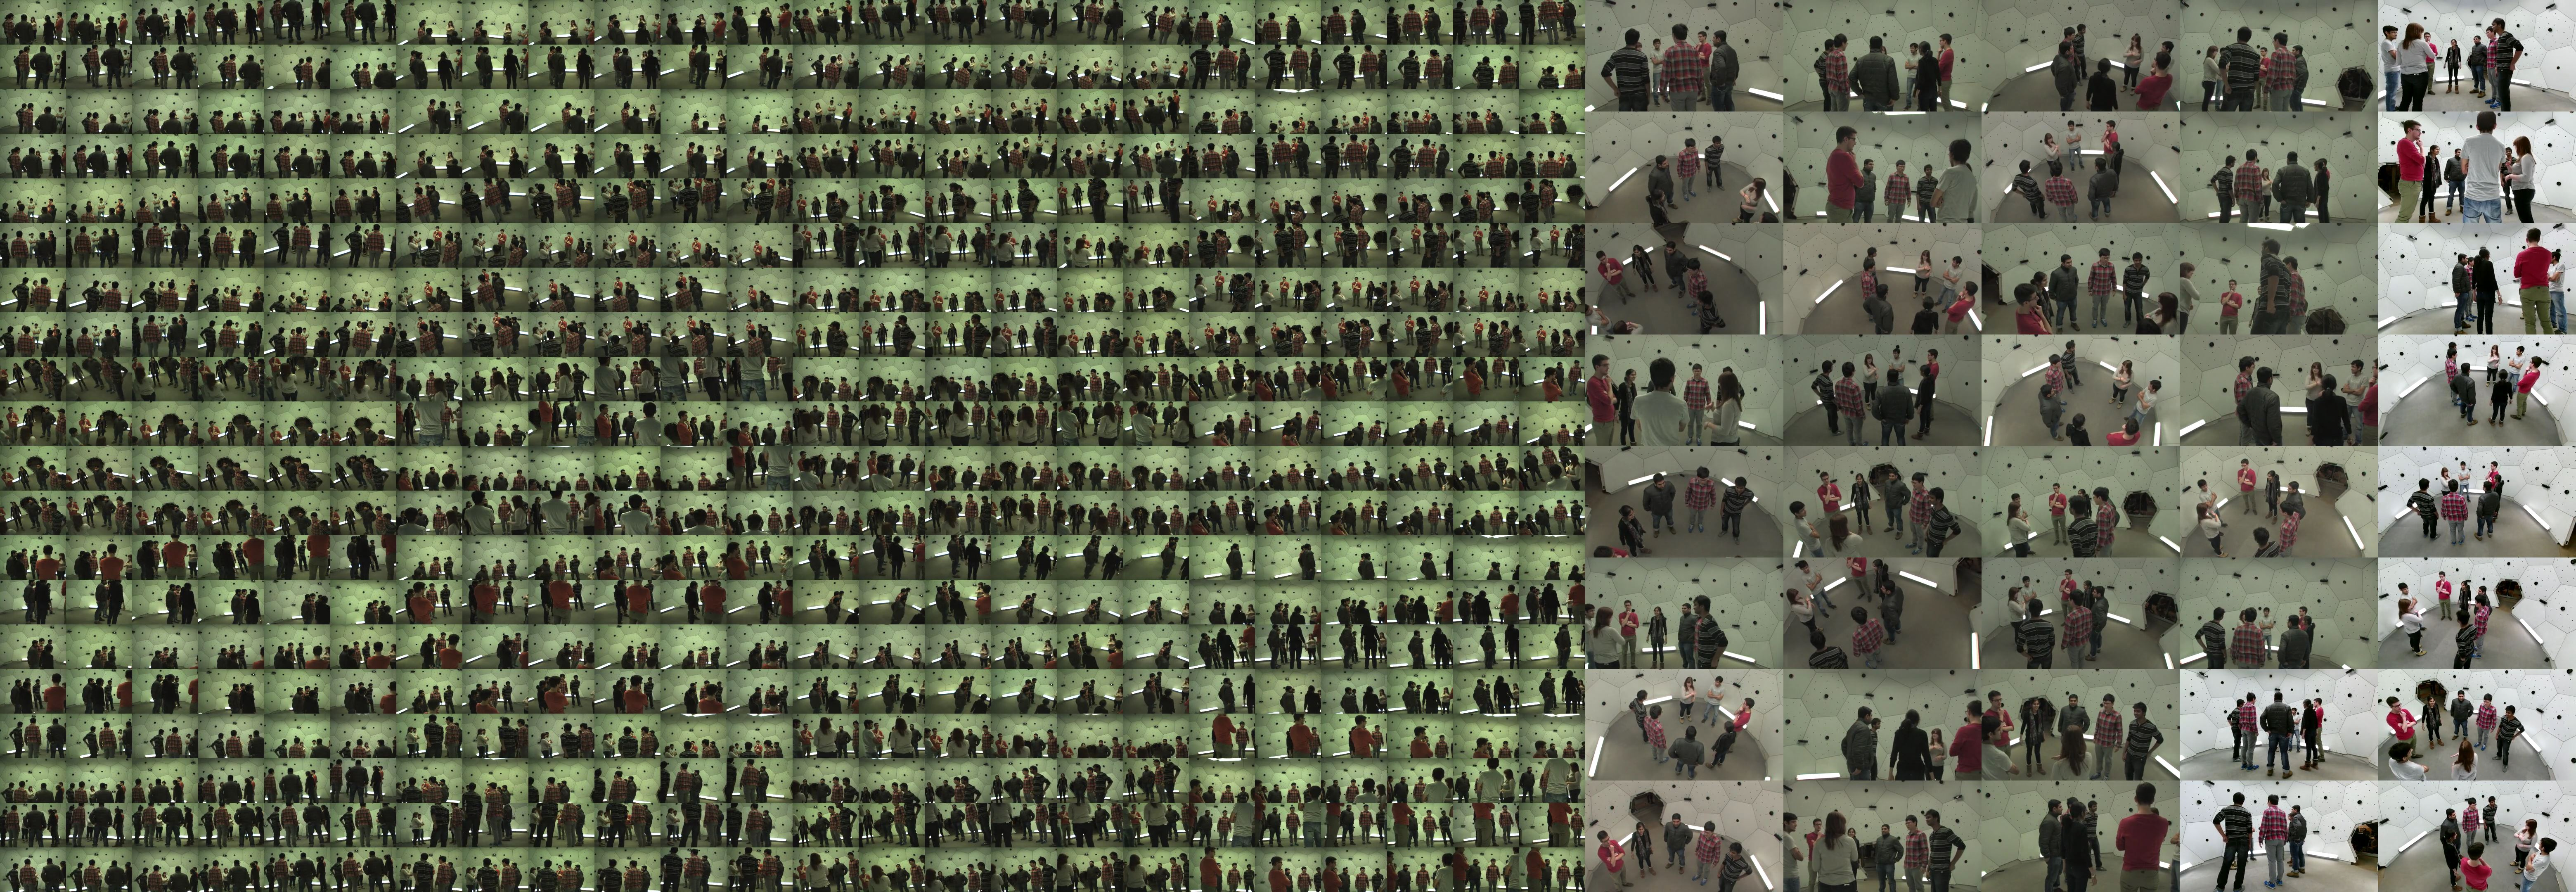
\includegraphics[width=\linewidth]{figures/Teaser}
%		\caption{521 unique views by 480 VGAs, 31 HDs, and 10 RGB+D sensors capturing a social interaction within the Panoptic Studio.} 
%		\label{fig:panopticviews}
%	\end{figure}


\begin{figure}[t]
	\centering
	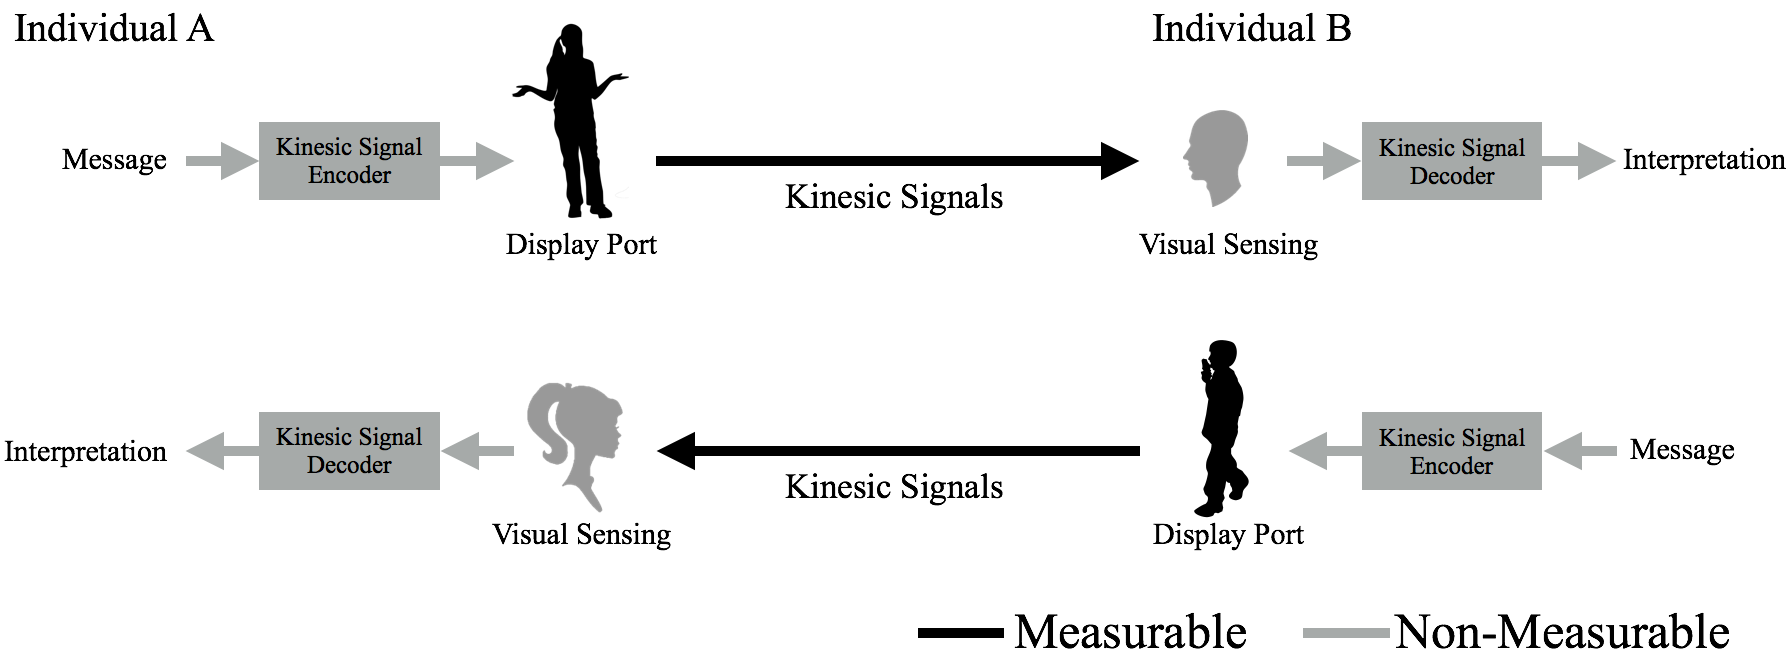
\includegraphics[trim=0 0 0 0, clip=true, width=\textwidth]{figures/kinesicflow2}
	\caption{Kinesic communication can be considered as an information flow among people. Messages are converted by an encoder and transmitted by our body as a form of kinesic signals. The transmitted signals are sensed, decoded, and finally interpreted by a receiver. We have no clear way to measure the flow or status inside our mind, but only can measure the exposed signals.}	
	\label{fig:kinesicflow}
\end{figure}


\section{Thesis  Summary}

The objective of this thesis is to develop a system to measure and model kinesic signals of interacting people. As a core contribution, we build a massively multiview system, the CMU Panoptic Studio, which is composed of 521 heterogeneous camera sensors, and present methods to measure dense 3D body surface movements, and subtle motion of 3D anatomical landmarks of full body including faces and hands. Example results are shown in the Figure~\ref{fig:teaser}. A large scale dataset capturing interactions of a large number of groups are collected and publicly released.

In the later part of the work, we address a framework to model kinesic signals as an information flow among people, by presenting a method to predict kinesic signals of an individual in a social situation. The goal is to build a model to mimic social communication of humans by producing appropriate response kinesic signals by receiving other people's kinesic signals as input. The model is trained using a Deep Neural Network with a large scale interaction dataset we have collected. A preliminary result in predicting gaze direction of a target individual given full body kinesic signals of others are presented. Additionally, we also present a preliminary result in quantifying the influence of each body part, which can be interpreted as a way to measure how a channel of signal contributes in kinesic communication. 

\subsection{Panoptic Studio: A Massively Multiview System (Chapter~\ref{chapter:system})}
The CMU Panoptic Studio is a system composed of 521 camera sensors. The system is specifically designed to overcome the sensing challenges emerging in social situations. The large number of views enables to release occlusions among interacting people, and densely cover the capture volume (5.49$m$ of a diameter) sufficient to have multiple people. The system is composed of three type of sensors: 480 VGA cameras, 31 HD cameras, and 10 RGB+D sensors. The VGA cameras are chosen to have more view points given the same pixel budget, while HD cameras are necessary to capture detailed structure of body such as faces and hands. RGB+D cameras make it easier to obtain a dense 3d point cloud at each time regardless the colors and textures of people. The combination of sensors contribute together in measuring kinesic signals at high resolution including the motion of 3D anatomical landmarks of full body, face, and hands, as well as measuring a dense 3D surface movement. 

We present a novel modularized design architecture to simplify the complexity of the system. The system is composed of repeated modules with the same shape and architecture, and each module is controlled by a separate local machine. This modularized design makes it easy to control and manage the system, and also enables efficient data acquisition by saving data locally. 

All cameras are accurately synchronized (or temporally aligned) by hardware clocks, and spatially calibrated in a common 3D world space. The core design choices and technical solutions including structural design, architecture, temporal calibration, and spatial calibration are addressed in Chapter~\ref{chapter:system}.

\subsection{Methods To Measure Total Body Kinesic Signals (Chapter~\ref{chapter:trajectory},~\ref{chapter:mocap},~\ref{chapter:totalcapture},~\ref{chapter:dataset})}

We present a method to measure various channels of subtle kinesic signals including 3D anatomical landmarks from body, face, hands and dense 3D body surface movements. The core goals in developing the methods are: (1) building a fully automatic method to capture social sequences at scale without human labors; (2) minimizing assumptions about scenes to be applicable in any type of motion and appearance of arbitrary number of people; and (3) avoiding intrusive approaches such as attaching artificial markers and avoiding a tedious 3D template building step. To this end, we present a method based on ``weak'' perceptual processes from the large number of views, and robustly measure kinesic signals by satisfying the aforementioned principles. In Chapter~\ref{chapter:trajectory}, a method to reconstruct dense surface movements, which we refer to as a ``trajectory stream", is presented by fusing optical flow cues from the large number of views in 3D. The core challenge of the method is to reason about a time varying visibility to fully exploiting the large number of views. In Chapter~\ref{chapter:mocap}, reconstructing the movement of 3D anatomical landmarks is presented. In this method, we run single image 2D detectors for body, face, and hands respectively in each view, and fuse them in 3D to reconstruct 3D locations of anatomical landmarks. By associating them with the trajectory stream, we obtain accurate markerless motion capture results, as well as semantic labeling of the trajectory stream.  In Chapter~\ref{chapter:totalcapture}, we present a 3D deformable human body model for total body motion capture which can express the full spectrum of body motions including facial expression and hand gestures in a unified parametric space. In Chapter~\ref{chapter:dataset}, we introduce a large scale dataset capturing and measuring hundreds of participants in various social situations. The dataset is currently publicly available in our dataset website. 


The relevant publication list for this thesis is as follows: 
\begin{itemize}
	\item  \noindent \href{http://www.cs.cmu.edu/~hanbyulj/14/CVPR_2014_Visibility.pdf}{``MAP Visibility Estimation for Large-Scale Dynamic 3D Reconstruction,"}\\ 
Joo et al, CVPR, 2014 (Oral) \href{https://www.youtube.com/watch?v=LaHTjBWago8}{(Video)}

\item \noindent \href{http://www.cs.cmu.edu/~hanbyulj/panoptic-studio/ICCV2015_SMC.pdf}{``Panoptic Studio: A Massively Multiview System for Social Motion Capture,"}\\ 
Joo et al, ICCV, 2015 (Oral) 

\item \noindent \href{https://ieeexplore.ieee.org/document/8187699}{``Panoptic Studio: A Massively Multiview System for Social Interaction Capture,"}\\ 
Joo et al, 2016 (an extended version of ICCV 2015, TPAMI 2017) \href{https://www.youtube.com/watch?v=m0-7HnWvxG4}{(Video)}

\item \noindent \href{https://arxiv.org/abs/1704.07809}{``Hand Keypoint Detection in Single Images using Multiview Bootstrapping ,"}\\ 
Simon, Joo, and et al, CVPR, 2017 \href{https://www.youtube.com/watch?v=Lajt6vS_dSM}{(Video)}	

\item \noindent \href{http://openaccess.thecvf.com/content_cvpr_2018/papers/Joo_Total_Capture_A_CVPR_2018_paper.pdf}{``Total Capture: A 3D Deformation Model for Tracking Faces, Hands, and Bodies,"}\\ 
Joo et al, 2016 (CVPR 2018, Best Student Paper Award) \href{https://www.youtube.com/watch?v=5QzdXQSf-oY}{(Video)}	

\item \noindent Panoptic Studio Database: \url{http://domedb.perception.cs.cmu.edu}


\end{itemize}

	
%\noindent \textbf{Proposed Work:} The current measurement results will be spatially and temporally improved by using temporal cues and dense point clouds from multiple RGB-D cameras. Our current method are presented for the goal in this thesis proposal, but it is not able to be applied to long-term sequences of our dataset due to the heavy computational cost. 

%\begin{figure}[t]
%	\centering
%	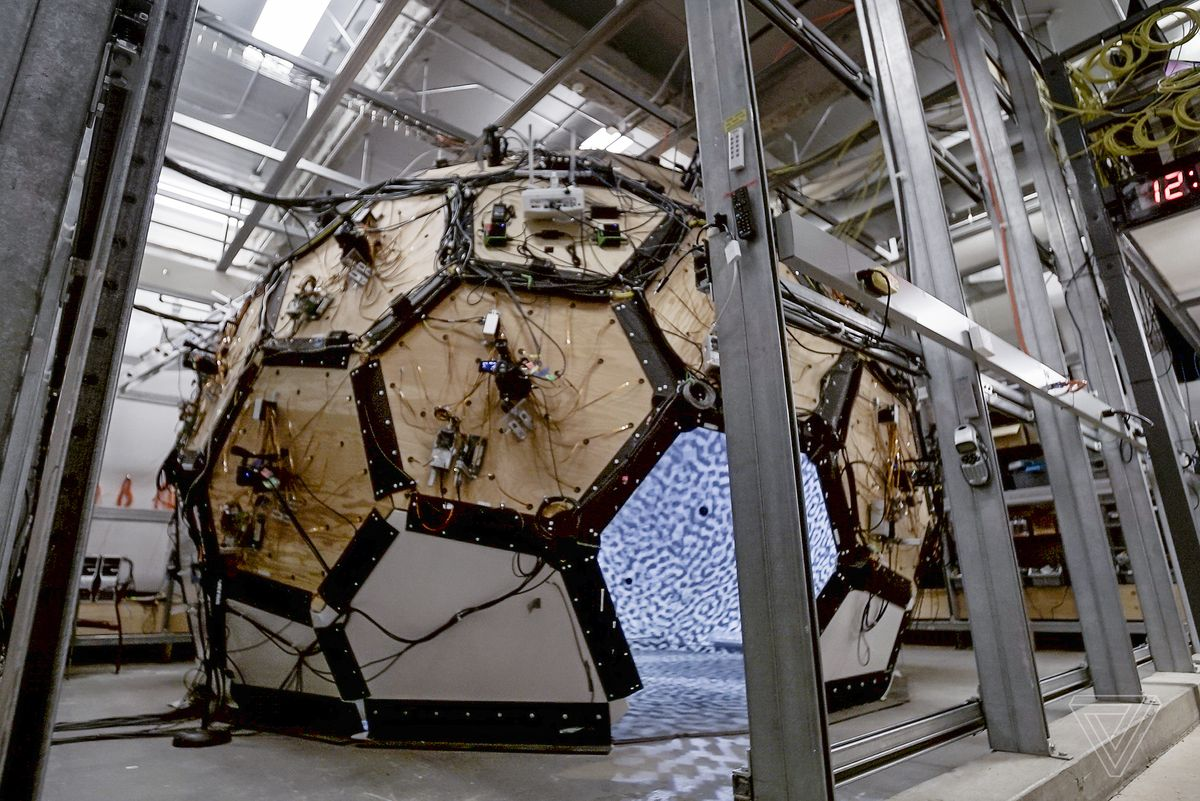
\includegraphics[trim=0 0 0 0, clip=true, width=0.32\textwidth]{figures/panoptic}
%	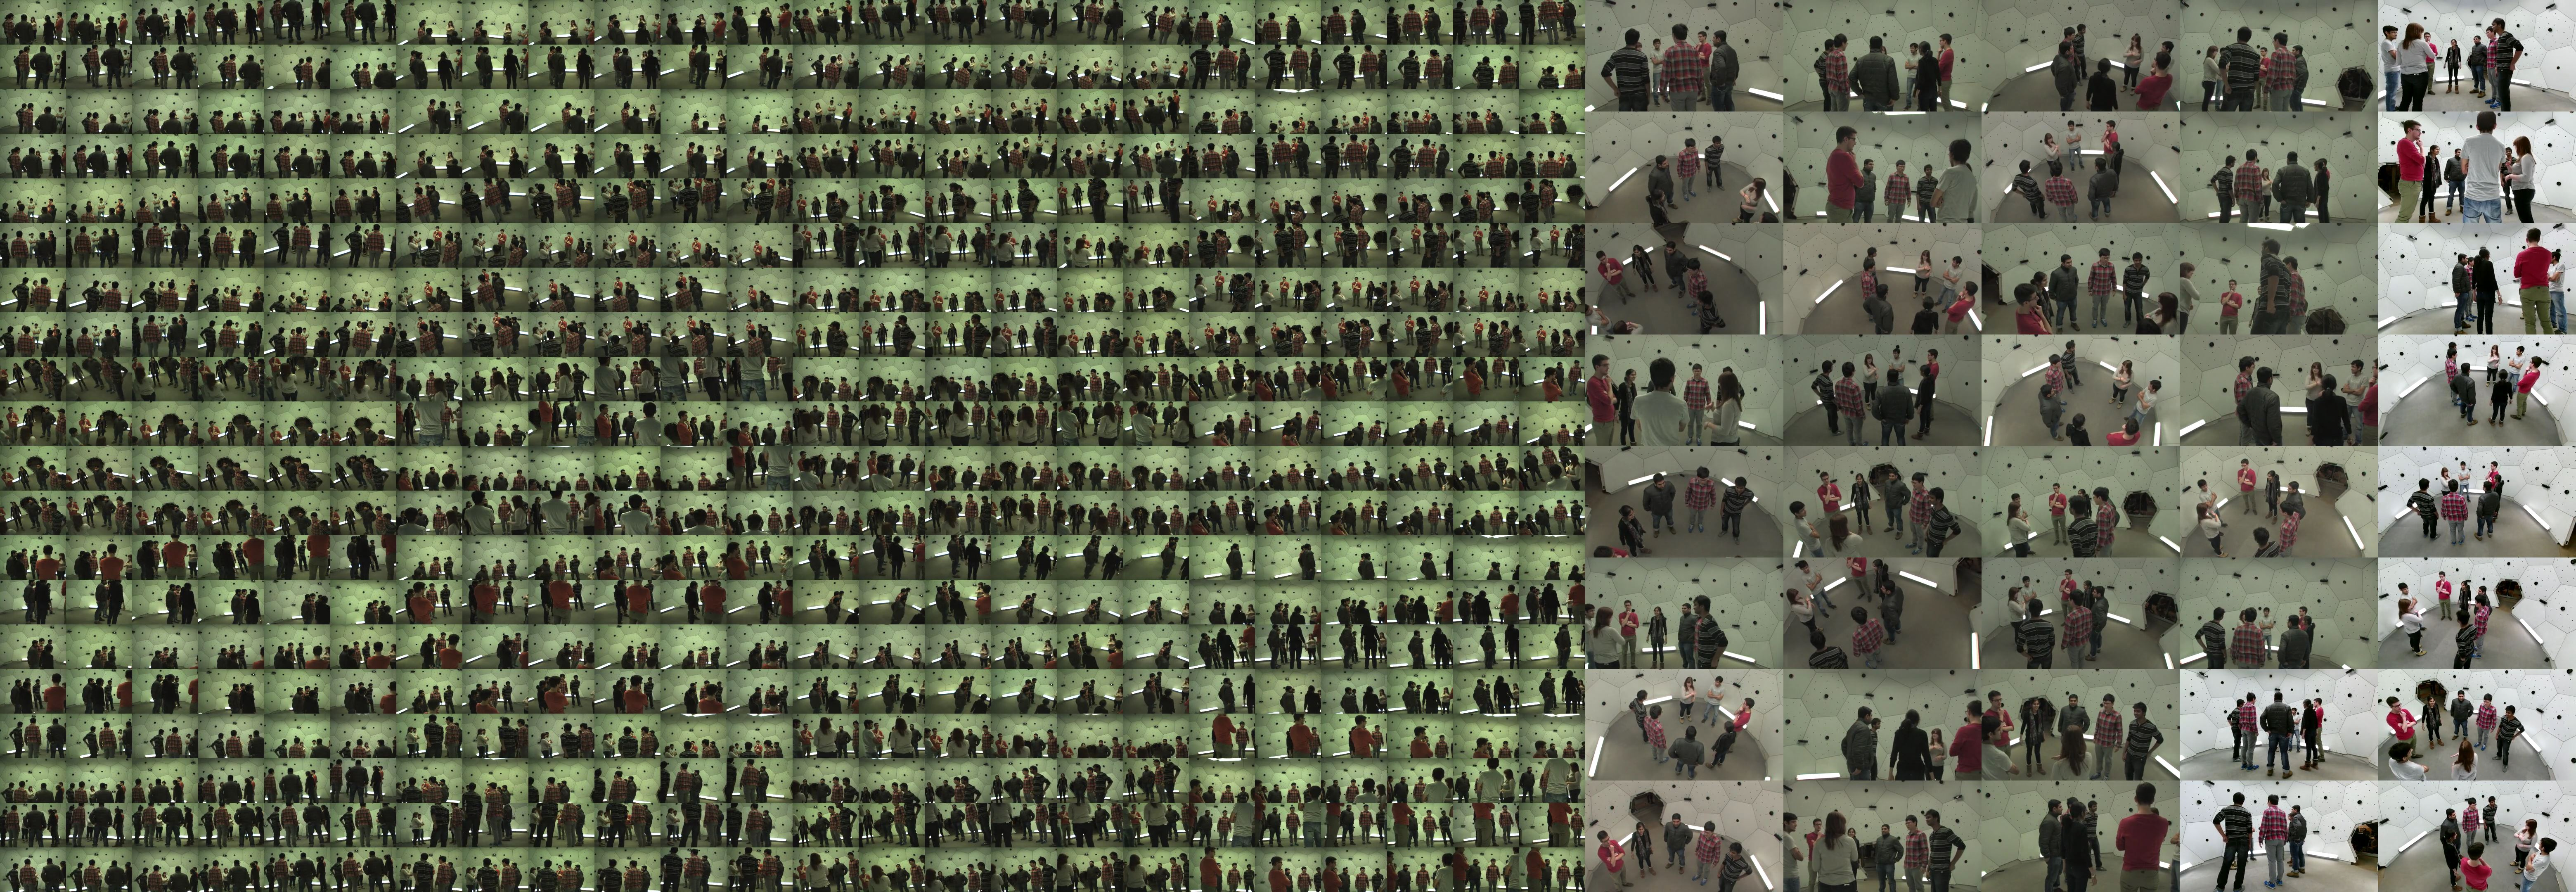
\includegraphics[width=0.62\textwidth]{figures/Teaser}\\
%	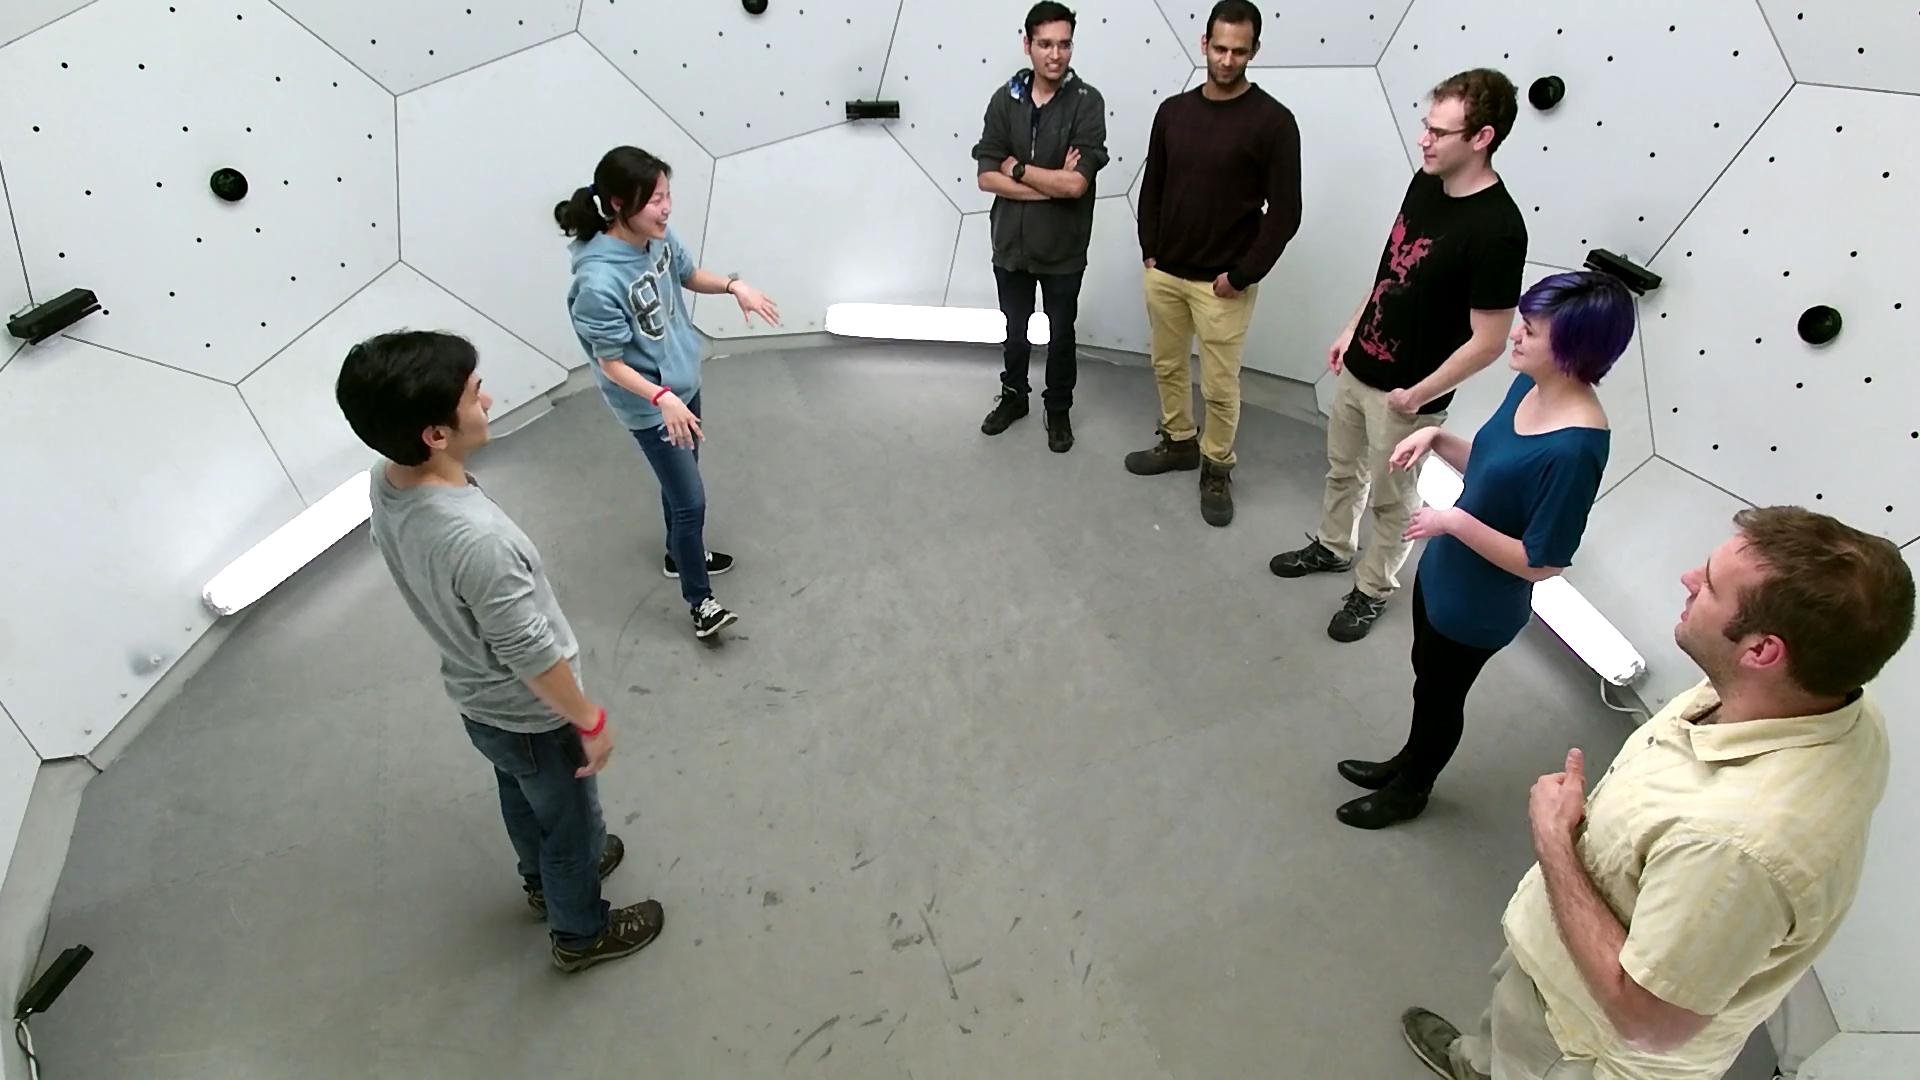
\includegraphics[trim=0 0 0 0, clip=true, width=0.311\textwidth]{figures/teaser_1}
%	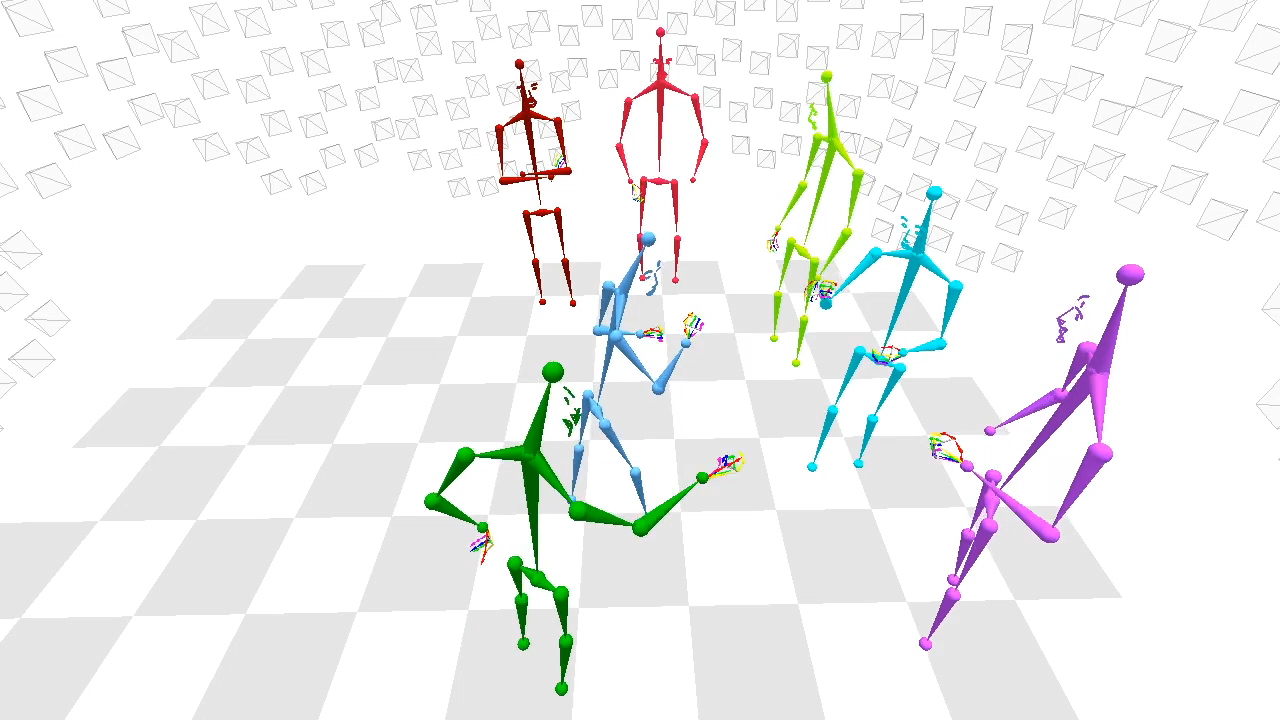
\includegraphics[trim=0 0 0 0, clip=true, width=0.311\textwidth]{figures/teaser_2}
%	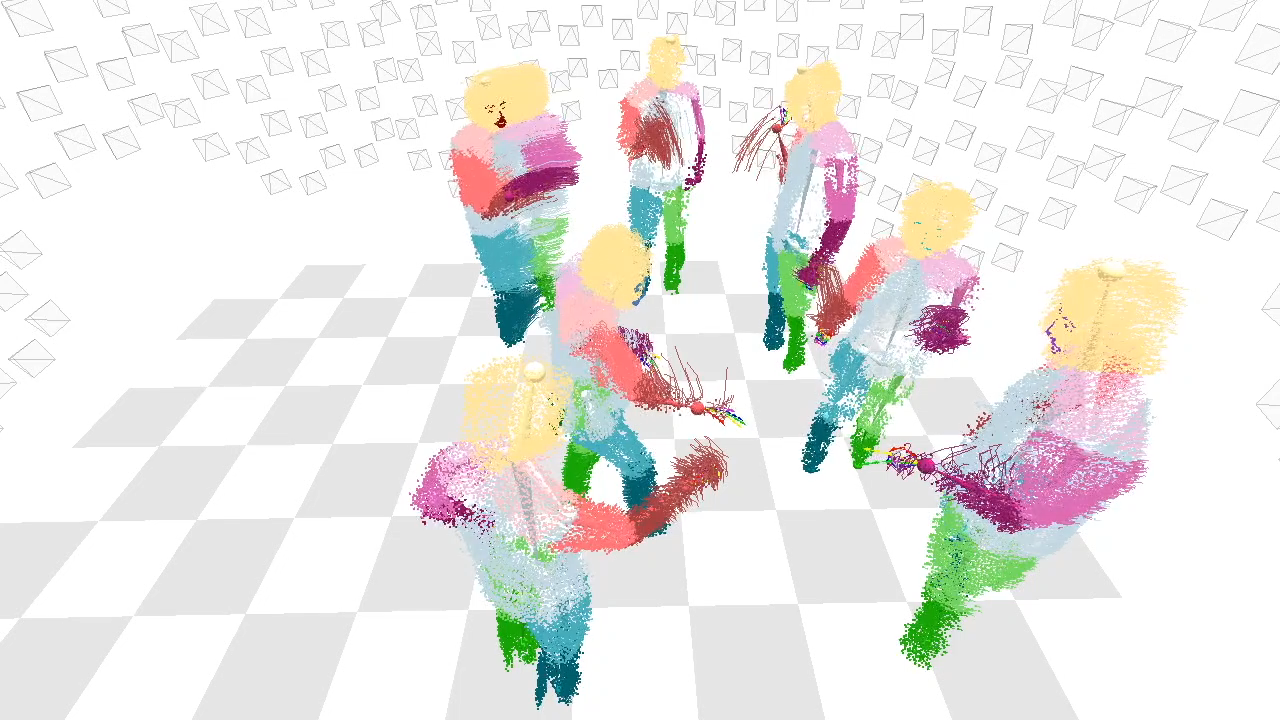
\includegraphics[trim=0 0 0 0, clip=true, width=0.311\textwidth]{figures/teaser_3}
%	\caption{(Top left) The Panoptic Studio, (Top right) 521 unique views by 480 VGAs, 31 HDs, and 10 RGB+D sensors capturing a social interaction within the Panoptic Studio, (Bottom) An example scene captured in the Panoptic Studio and measured kinesic signals.}	
%	\label{fig:teaser}
%\end{figure}


\begin{figure}[t]
	\centering
	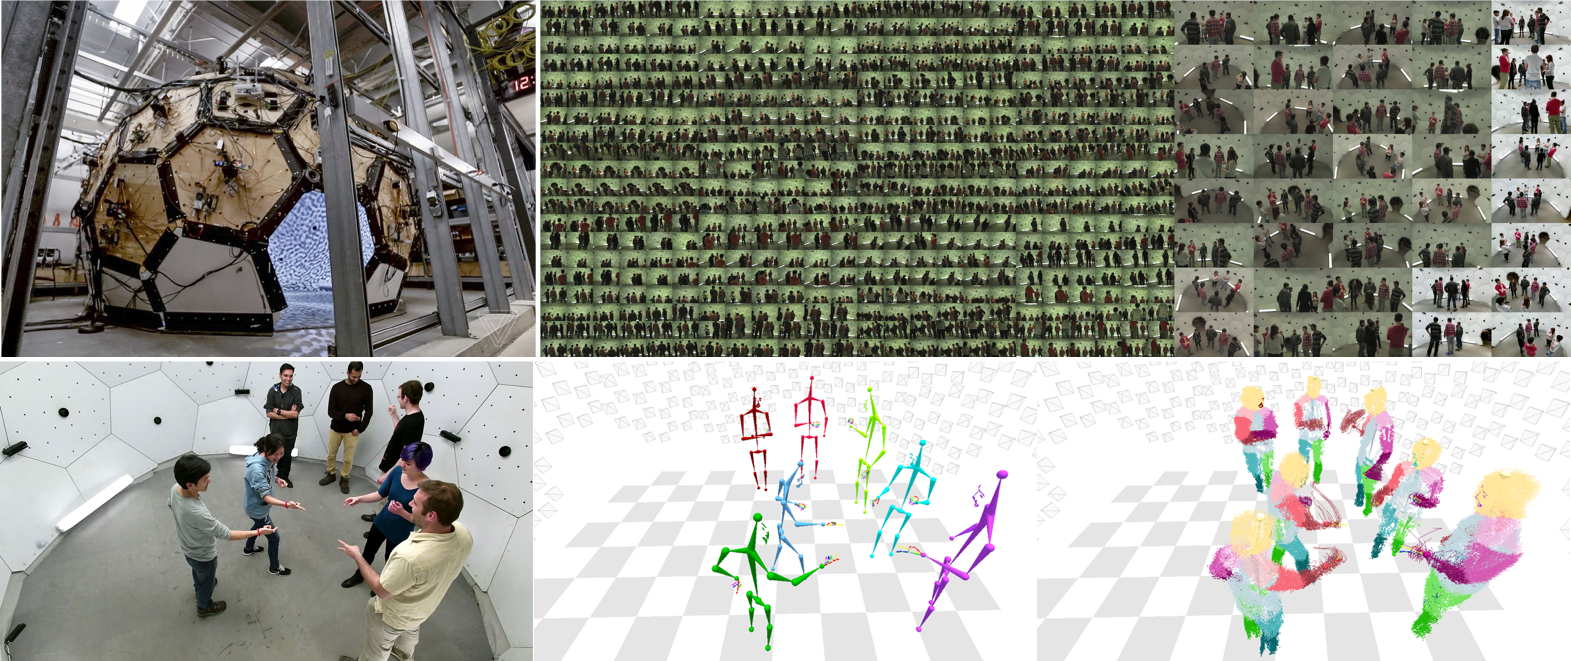
\includegraphics[width=\textwidth]{figures/teaser_full}
	\caption{(Top left) The Panoptic Studio; (Top right) 521 unique views by 480 VGAs, 31 HDs, and 10 RGB+D sensors capturing a social interaction within the Panoptic Studio; (Bottom left) An example scene captured in the Panoptic Studio; (Bottom center) Measured anatomical landmarks from bodies, faces, and hands; and (Bottom right) Measured motion of dense 3D surface points of multiple people.}	
	\label{fig:teaser}
\end{figure}


\subsection{Methods To Model Kinesic Signals In Social Interactions (Chapter~\ref{chapter:prediction})  }

We present a method to continuously predict high dimensional kinesic signals in social situations based on a data driven way. Our model takes kinesic signals emitted by others as input, and produces kinesic signals of the target individual as output. Conceptually, our model regresses a decoder and an encoder in Figure~\ref{fig:kinesicflow} together in a single optimization function, where the decoder interprets the conveyed messages in kinesic signal from others and the encoder transmits the message of target person through kinesic signals. The core advantage of our model is that its input and output are defined by objectively measurable signals, without requiring the representation of semantic meaning of them. Our model is built using a Deep Neural Network, and trained by the large scale dataset collected by our Panoptic Studio. Importantly, our model also enables to measure the importance of each body signal in a social communication, quantifying accuracy by eliminating each part signal. The detailed method and preliminary results are presented in Chapter~\ref{chapter:prediction}.

%%%%%%%%%%%%%%%%%% Old intro starts %%%%%%%%%%%%%%%%%% 
%During social communications, we use nonverbal signals to transmit messages and intents that cannot be conveyed with words. For example, it is commonly accepted by social psychologists that much of the emotional meaning is expressed via nonverbal signals \cite{Mehrabian67, Mehrabian81, Birdwhistell70, Moore13}. 
%Nonverbal signals include not only facial expressions and body gestures (also called Kinesics~\cite{Birdwhistell70}), but also all types of ``other-than-words" channels used in communications, including distance between people (e.g., proxemics~\cite{Hall66}), relative position (e.g., F-formation \cite{kendon90}), prosody, physical appearance, haptics, and so on. Interestingly, although we are very familiar with how to use these signals, the underline protocol is still very poorly understood---Sapir~\cite{Sapir-1949} called it ``an elaborate code that is written nowhere, known to no one, and understood by all". Such limited knowledge makes it difficult to transfer the ability of nonverbal communication to machines and robots, and therefore, machines that can convincingly interacting socially with humans do not currently exist. 
%
%Drawing an analogy to telecommunication systems, nonverbal communications also involve senders, receivers, and a ``protocol" to pass messages, where the protocol represents a system of rules to encode and decode the transmitted information via measurable signals. A possible way to decipher the nonverbal code is then by directly modeling the encoder and decoder, based on observed data. For example, happiness and joyfulness can be encoded into a smiling signal expressed by facial muscles. If it were possible to collect a large amount of mappings between the measured nonverbal signals and the transmitted semantic meanings, the protocol could be modeled using a supervised learning technique. In the study of verbal communication, this approach can be applicable. Speech can be transformed (encoded) to languages without ambiguity or losing information. It also follows strict grammatical rules and is composed of well-defined elements, words and phonemes. Once they are transformed into languages they are mostly ready to be further processed to better understand communications.  
%
%
%Much of the nonverbal communication work to date is based on the similar approach (e.g., facial expression database collected by asking subjects to perform a series of predetermined expressions~\cite{de2011facial}), it is comparatively far less understood. The major limitation of this direction is the fact that there is no way to correctly label the messages transmitted via nonverbal signals. The signals are on a continuous space mixed by multiple high dimensional channels, and thus a large amount data is missing if we simply label or describe them by words in discrete levels. Thus, there is no good way to transform the signals to the data to be processed other than saving the signals themselves. 
%
%Three major challenges arise: (1) How to capture social signals; (2) How to measure social signals; and (3) How to understand social signals. First, the social signal can be only captured by observing interacting people in natural scenarios. However, there are principal challenges in capturing social signaling between individuals in a group: (1) social interactions have to be measured over a volume sufficient to house a dynamic social group, yet subtle details of the motion where important social signals are embedded must be captured; (2) strong occlusions emerge functionally in natural social interactions (e.g., people systematically face each other while interacting, bodies are occluded by gesticulating limbs); (3) human appearance and configuration variation is immense; and (4) social signaling is sensitive to interference---for instance, attaching markers to the face or body, a pre-capture model building stage, or even instructing each individual to assume a canonical body pose during an interaction, primes the nature of subsequent interactions. To avoid these obstacles many of previous work restrict the scenarios to a table setup where people are sitting on chairs by limiting their bodily movements~\cite{alameda2016salsa, mccowan2005ami, lepri2012connecting}.
%
%Second, how to measure social signals from recorded videos is not straightforward. To be ideal, stereo images as human does can be used as the input of the system to mimic human's social interaction. However, this basically means that the system should hand all the perception processes as they are performed in humans' brain. Instead, we may consider to extract ``semantic" signals from raw videos, and they including facial expression and body motion, which can be easier to be further processed. However, this also requires to solve multiple fundamental problems in computer vision. 
%
%Third, how to understand the nonverbal communication is largely unexplored area. The major limitation of pursuing such direction is the fact there is no large scale data where model can be trained. Studies to understand human motions are usually based on single person's motion only~\cite{mnih2012conditional, Fragkiadaki_2015_ICCV, jain2016structural}. Otherwise, the previous work is usually based on modeling encoder between the manually annotated labels and coarse signals (which contains the ``biased labeling problem" mentioned above). To be objectively understand the communication, the model should be based on ``observed" signals only which can be measurable by systems.
%
%
%To address these challenges, we develop the ``Panoptic Studio", a novel multiview camera system equipped with 480 VGA cameras, 31 HD cameras, 10 RGB+D cameras, and multiple microphones. This massively multiview system can directly release many capture challenges including covering a large volume, and handling occlusions. There are multiple issues to be carefully considered to design such a big system including synchronization, calibration, capturing system, machine communications, and so on. In this thesis, all the design aspect of the Panoptic Studio is addressed as the results of multiple years of collaboration of several contributors. This paper also address the way to extract various social signals (joint landmarks, facial landmarks, finger landmarks, and dense surface trajectory streams). The core idea in measuring this social signals is based on relatively ``weak" measurement from each view but relying on a large number of views, rather than relying on a complicated template model with strong prior assumption about this scenes. In this thesis, the method and demonstration to measure subtle details of social signals in a fully automatic ways are presented. 
%
%An essential part to understand nonverbal behavior is based on a large scale data. As a core part of this thesis, a large scale dataset is captured and measure using our system. To share the dataset to public, we also build to a system to efficiently share the date to all the research communities. Several aspect in designing the system and dataset is also addressed. More importantly, we scale up the data size in the unprecedented level by inviting hundreds of participants. The game protocol is also carefully designed with a close collaboration psychologists.
%
%As the last chapter of this thesis, we present a method to understand nonverbal communication based on measurable signals. In contrast to the previous work which tries to model the ``encoder" between the message to signal directly, we only use the ``objectively" measurable signal without requiring biased human annotations. To this end, we introduce a novel research problem, \emph{Social Signal Prediction}, problem and study the impact of social signals in predicting future motion of the target humans.  
%%%%%%%%%%%%%%%%%% Old intro ends %%%%%%%%%%%%%%%%%% 
%
%
%\begin{figure}[t]
%	\centering
%	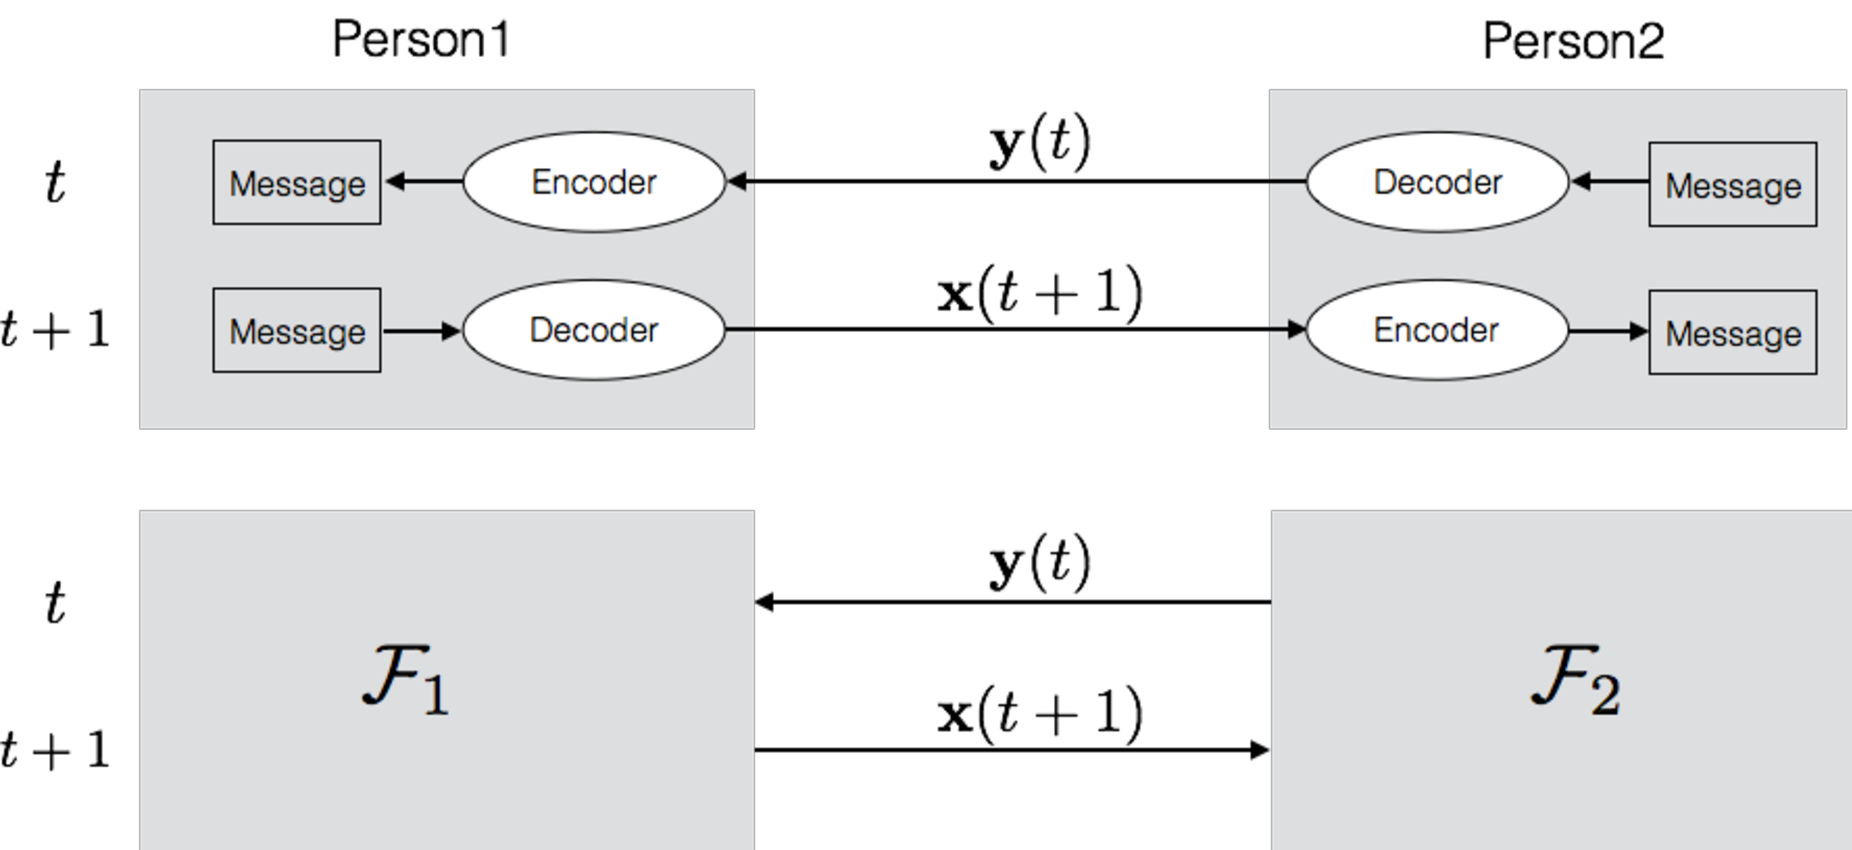
\includegraphics[trim=0 0 0 0, clip=true, width=0.5\columnwidth]{figures/encodDecod2}
%	
%	\caption{Encoder and Decoder model of Social Signals}	
%\end{figure}

%\begin{itemize}
%	\item Motivation: Nonverbal social signals play important role in social communication, transmitting rich information which cannot be conveyed by languages. 
%	\item They are still poorly understood. Why?
%	\item Challenges
%		\subitem - Measurement: large volume, occlusions, immense pose configuration, priming issue (requiring a markerless method).
%		\subitem - Understanding (prediction): high dimensional, hard to model by a hand-crafted way, no available large scale data for ``natural" social interactions, no previous work based on a data-driven method. 
%	\item Our approach
%		\subitem - We present a new capture system and method using massively multiple views: social interaction should be measured by fusing lots of (simple) measurements, rather than complicated methods with a few views
%		\subitem - We present a new data-driven method to model socially interacting multiple people's motion: the model should be trained using a large scale data capturing ``natural" social interactions
%
%\end{itemize}


%\section{Notation}

%During social communication, people use nonverbal body signals using their body movement and facial expression to transmit their intent and emotion. The convey signals have richer information which cannot be conveyed by just using verbal cues. This signal plays very important role, but poorly understood up to now. 

%
%Despite the fundamental role nonverbal cues play in enabling social function~\cite{Birdwhistell-1970,Philpott-1983}, the protocol underlying this communication is poorly understood---Sapir~\cite{Sapir-1949} called it ``an elaborate code that is written nowhere, known to no one, and understood by all". Some structures of this code have been identified through observational study, such as reciprocity~\cite{Brazelton-1974} or synchrony~\cite{Condon-1974}. However, systematic studies of such phenomena have remained almost entirely focused on the analysis of facial expressions, despite emerging evidence~\cite{Meeren-2005,Aviezer-2012} that facial expressions provide a fundamentally \emph{incomplete} characterization of nonverbal communication. One proximal cause for this singular focus on the face is that capturing natural social interaction presents challenges that current state-of-the-art motion capture systems simply cannot address. This paper describes an approach to capture social signals in natural human interactions, presenting fundamental innovations that span capture design architecture, motion reconstruction algorithms, and a large scale dataset capturing more than 3 hours of group interaction scenes using 521 heterogeneous sensors.
%
%There are four principal challenges in capturing social signaling between individuals in a group: (1) social interactions have to be measured over a volume sufficient to house a dynamic social group, yet subtle details of the motion where important social signals are embedded must be captured; (2) strong occlusions emerge functionally in natural social interactions (e.g., people systematically face each other while interacting, bodies are occluded by gesticulating limbs); (3) human appearance and configuration variation is immense; and (4) social signaling is sensitive to interference---for instance, attaching markers to the face or body, a pre-capture model building stage, or even instructing each individual to assume a canonical body pose during an interaction, primes the nature of subsequent interactions. 
%
%In this paper, we present a system designed to address these issues, with integrated innovations in hardware design, motion representation, and motion reconstruction. The organizing principle is that social motion capture should be performed by the consolidation of a large number of ``weak" perceptual processes rather than the analysis of a few sophisticated sensors. The large number of views provide robustness to occlusions, provide precision over the capture space, and facilitate the boosting of weak 2D human pose detectors into a strong 3D skeletal tracker without any prior about the scenes and subjects. In particular, our contributions include: 
%
%	1) \textbf{Modularized Hardware}: We present the modular design of a massively multiview capture consisting of 480 VGA cameras, 31 HD Cameras, and 10 Kinect v2 RGB+D sensors, distributed over the surface of geodesic sphere with a 5.49m diameter (sufficient to house social groups).  %simultaneously triggered/accurate time aligned
%	
%	2) \textbf{3D Motion Reconstruction Algorithm for Interaction Capture}:  We present a method to automatically reconstruct full body motion of interacting multiple people. Our method does not rely on a 3D template model or any subject-specific assumption such as body shape, color, height, and body topology. Yet, our method works robustly in various challenging social interaction scenes of arbitrary number of people, producing temporally coherent time-varying body structures. Furthermore, our method is free from error accumulation and, thus, enables capture of long term group interactions (e.g., more than 10 minutes). 
%	%Our system does not require subjects to: (1) perform any predefined pose for initial alignment; (2) wear clothings with distinctive color from others, (3) directly face sensors to get reasonable measurements; (4) restrict the in-group movement of subjects. All these benefits are key to enabling the study of social interactions at scale. 
%	
%%	3) \textbf{Skeletal Representation}: We present a new representation for social motion capture labeling and embedding a dense 3D trajectory stream within a moving skeletal frame for each individual.
%	%	\item \textbf{3D Motion Reconstruction Algorithm}: We present a novel algorithm, inspired by boosting approaches, for fusing ``weak" human pose detection in each view with 3D tracking, to estimate the articulated nonrigid representation across the diverse set of views
%	%Our algorithm is designed to capture the motion of arbitrary (unknown) number of multiple people, without making prior assumptions about the subjects such as their body shape, texture, and measurement of bone length. Thus, we do not require a predefined model for each individual, or require participants to assume a canonical body pose for initialization during capture. 
%	
%	3) \textbf{Social Interaction Dataset}: We publicly share a novel dataset which is the largest in terms of the number of views (521 views), duration (3+ hours in total), and the number of subjects in the scenes (up to 8 subjects) for full body motion capture. Our dataset is distinctive from the previously presented datasets in that ours captures natural interactions of groups without controlling their behavior and appearance and contains motions with rich social signals as shown in Figure~\ref{fig:iconicPoses} (right). The system described in this paper provides empirical data of unprecedented resolution with the promise of facilitating data-driven exploration of scientific conjectures about the communication code of social behavior. All the data and output are publicly shared on our website\footnote{ \url{https://domedb.perception.cs.cmu.edu}}. 
%	
	
%	
%\section{Proposal Summary}
%\subsection{Completed Work to Data}
%\subsection{Proposed Work}
%\subsection{Timeline}
%\section{Notations}
%
%\section{Multiview System}
%\section{Markerless Motion and Face Capture}
%\section{Social Signal Processing}
%\section{Overview of Contributions}
%\subsection{Timeline}
%\begin{figure}[!ht]
%	\centering
%	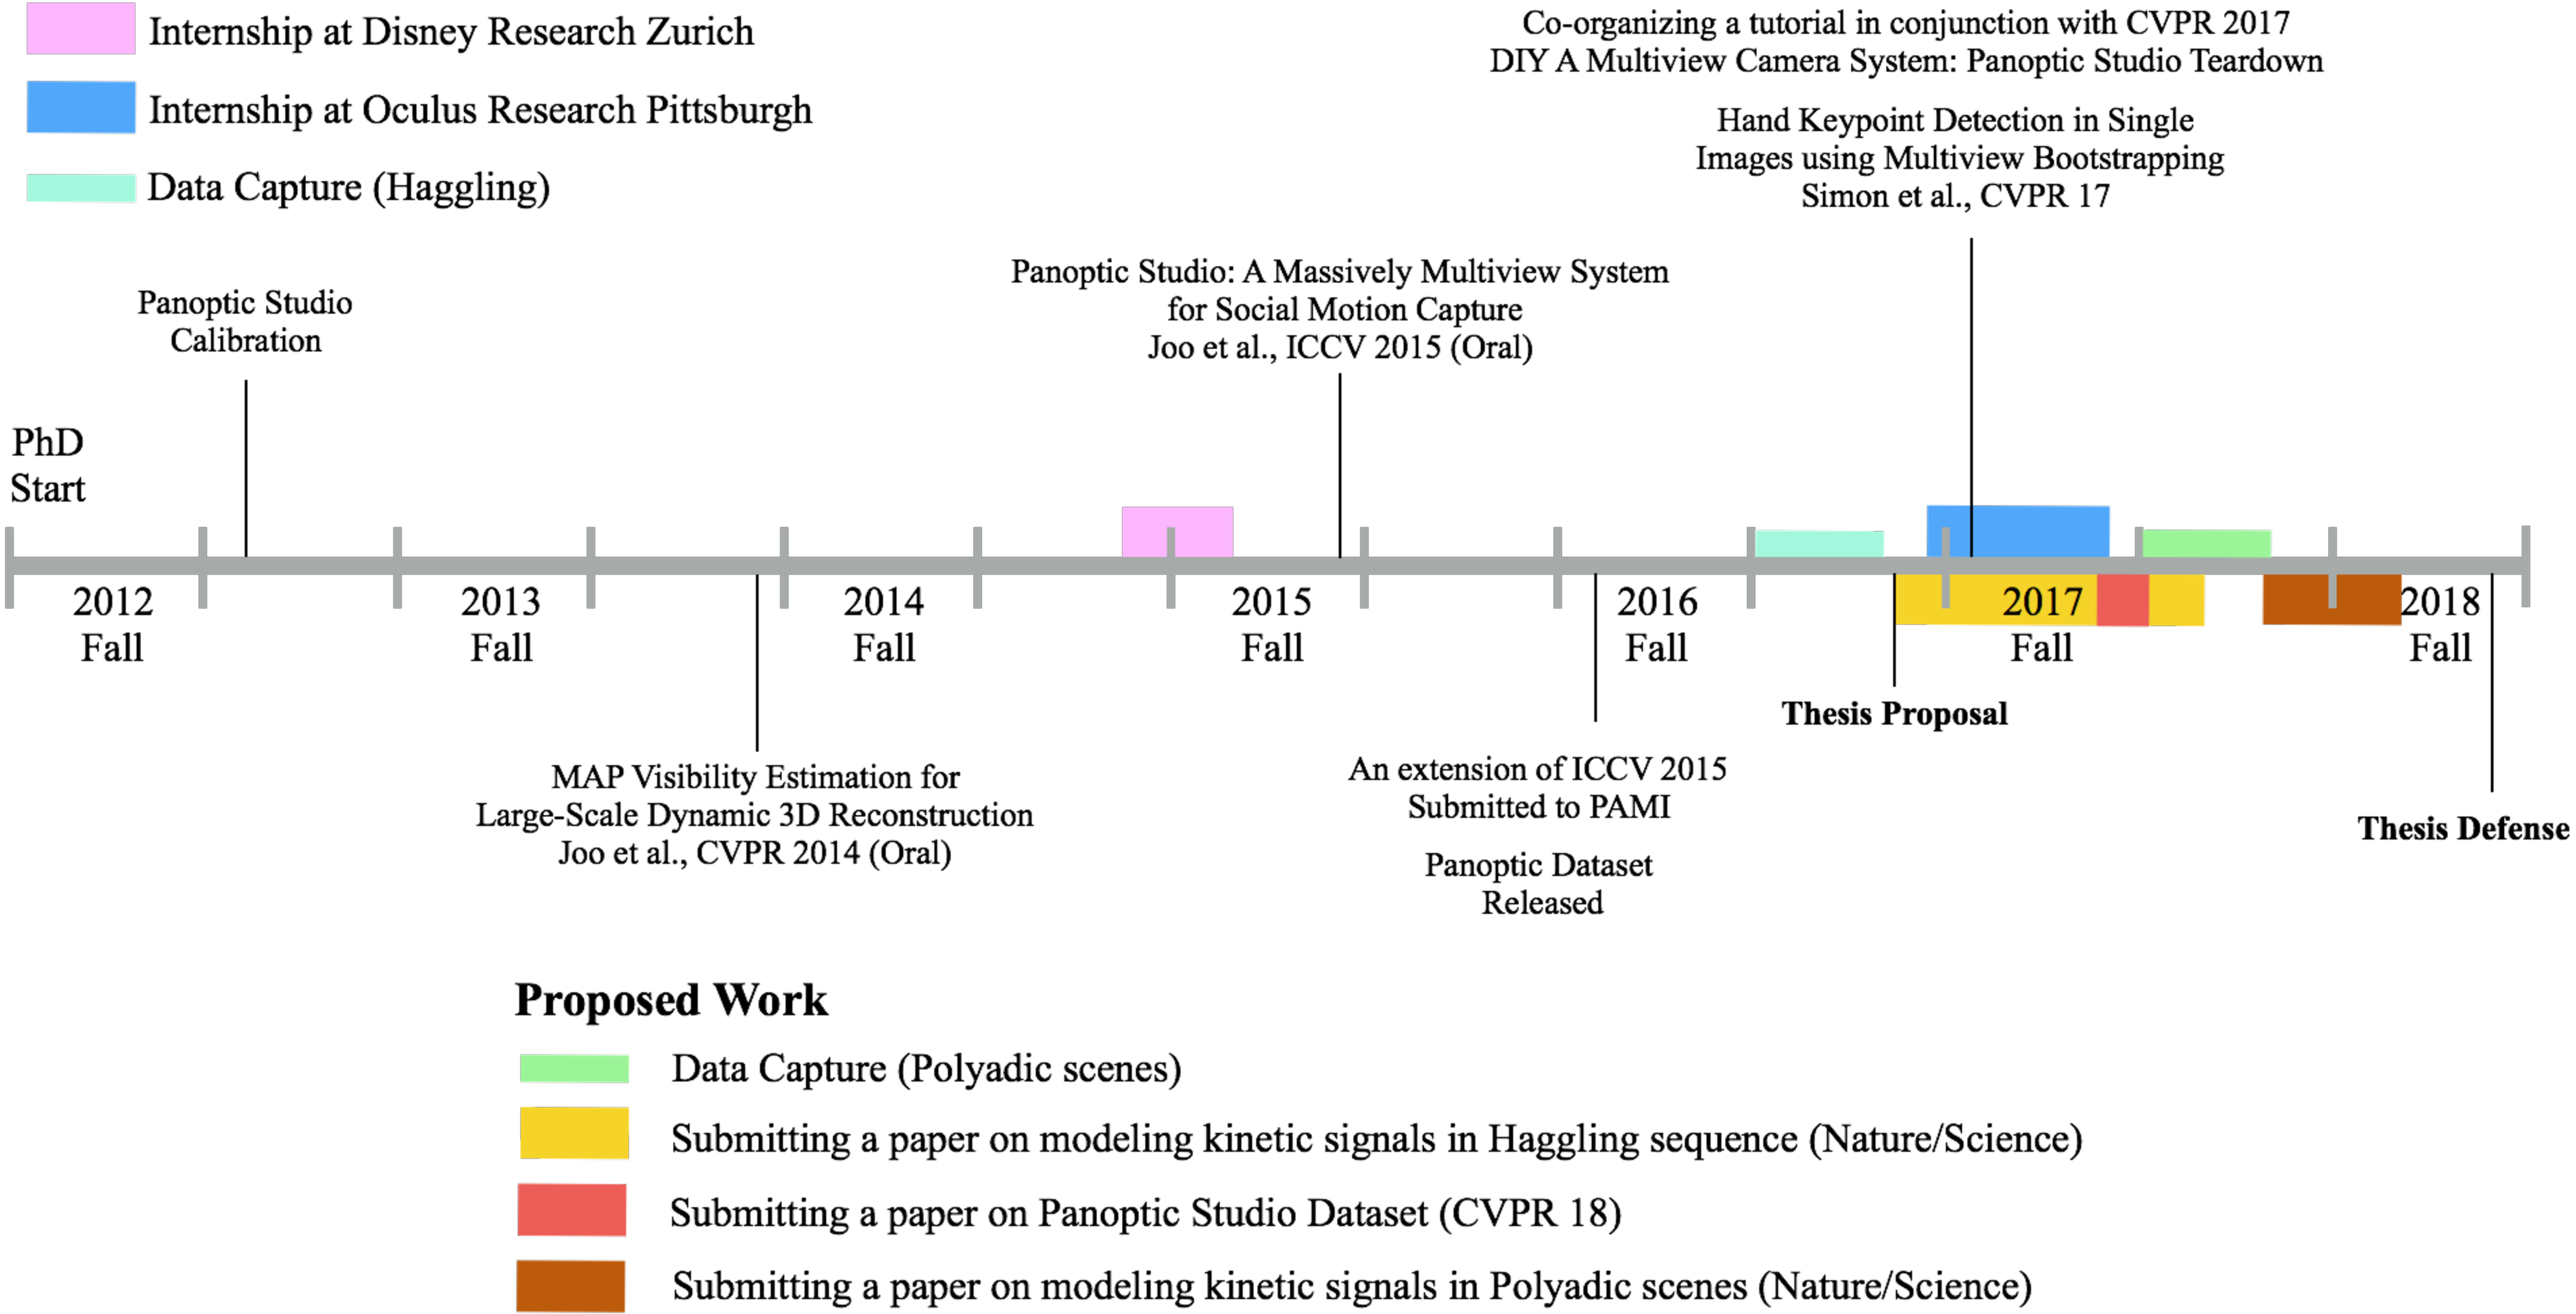
\includegraphics[trim=0 0 0 0, clip=true, width=0.95\textheight,angle=270,origin=c]{figures/timeline}
%%	\caption{A Timeline}	
%	\label{fig:timeline}
%\end{figure}

\newpage 